\documentclass{article}
\usepackage{listings}
\usepackage{graphicx}
\usepackage{graphicx}
\usepackage{subfigure} 
\title{Operational Statistics for SAR Imagery Report}
\author{Guanchun Wang}
\date\today


\begin{document}
	\maketitle
	
	\section{sample Image}
	\begin{lstlisting}[frame=tb]
	
	> imagepath <- "../Data/Images/ESAR/"
	
	> HH_Complex <- myread.ENVI(paste(imagepath,
	"ESAR97HH.DAT", sep = ""),
	paste(imagepath, "ESAR97HH.hdr", sep = ""))
	> HH_Intensity <- (Mod(HH_Complex))^2
	> example <- HH_Intensity[256:356,256:356]
	> vexample <- data.frame(HH=as.vector(example))
	> summary(vexample)
	HH
	Min.   :     107
	1st Qu.:   97227
	Median :  269012
	Mean   :  516138
	3rd Qu.:  624278
	Max.   :10068006
	> plot(imagematrix(equalize(example))) (figure.a)
	\end{lstlisting}
	\begin{figure}[htbp]
		\centering
		\subfigure[example.]{
			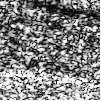
\includegraphics[width=5.5cm]{example.jpg}
			%\caption{fig1}
		}
		\quad
		\subfigure[HistogramExample.]{
			\includegraphics[width=5.5cm]{HistogramExample(1).pdf}
		}
		\quad
		\subfigure[HistogramRestrictedExample.]{
			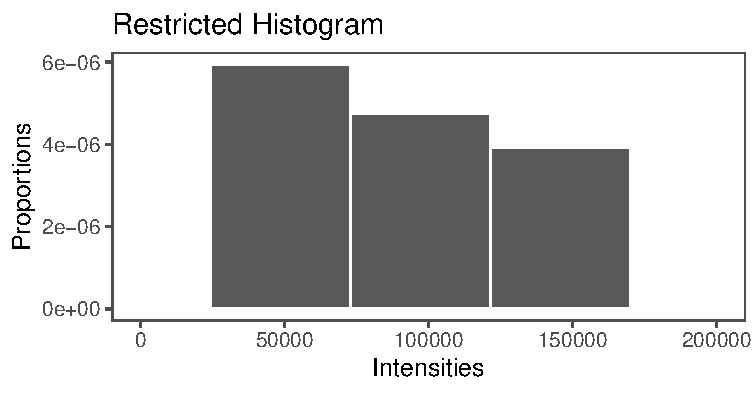
\includegraphics[width=5.5cm]{HistogramRestrictedExample.pdf}
		}
	\end{figure}
	
	\section{Histogram}
	\begin{lstlisting}[frame=tb]
	> ggplot(data=vexample, aes(x=HH)) +
	+   geom_histogram(aes(y=..density..),
	+                  binwidth = binwidth_complete) +
	+   xlab("Intensities") +
	+   ylab("Proportions") +
	+   ggtitle("HistogramExample") +
	+   theme_few()
	\end{lstlisting}
	
	\section{Estimation}
\subsection{analogy}
\begin{lstlisting}[frame=tb]
> GI0.Estimator.m1m2 <- function(z, L) {
+   m1 <- mean(z)
+   m2 <- mean(z^2)
+   m212 <- m2/m1^2
+
+   a <- -2 - (L+1) / (L * m212)
+   g <- m1 * (2 + (L+1) / (L * m212))
+
+   return(list("alpha"=a, "gamma"=g))
+ }
\end{lstlisting}
\begin{lstlisting}[frame=tb]
> estim.example <- GI0.Estimator.m1m2(example, 1)
> estim.example
$alpha
[1] -2.653035

$gamma
[1] 1369331
\end{lstlisting}
\subsection{Likelihood}
\begin{lstlisting}[frame=tb]
> LogLikelihoodLknown <- function(params) {
+
+   p_alpha <- -abs(params[1])
+   p_gamma <- abs(params[2])
+   p_L <- abs(params[3])
+   n <- length(z)
+   return(
+     n*(lgamma(p_L-p_alpha) - p_alpha*log(p_gamma)
- lgamma(-p_alpha)) +
+       (p_alpha-p_L)*sum(log(p_gamma + z*p_L))
+   )
+ }
\end{lstlisting}
\begin{lstlisting}[frame=tb]
> estim.exampleML <- maxNR(LogLikelihoodLknown,
+			start=c(estim.example$alpha,
+			estim.example$gamma,1),
+			activePar=c(TRUE,TRUE,FALSE))$estimate[1:2]
> estim.exampleML
[1] -3.687864e+00  1.369304e+0
\end{lstlisting}

\end{document}

